% Generated 2021-08-25 18:02:22 +0530
\subsection{DataItems} \label{sec:DataItems}


\block{DataItems} \glspl{organize} \block{DataItem} elements.

\begin{figure}[ht]
  \centering
    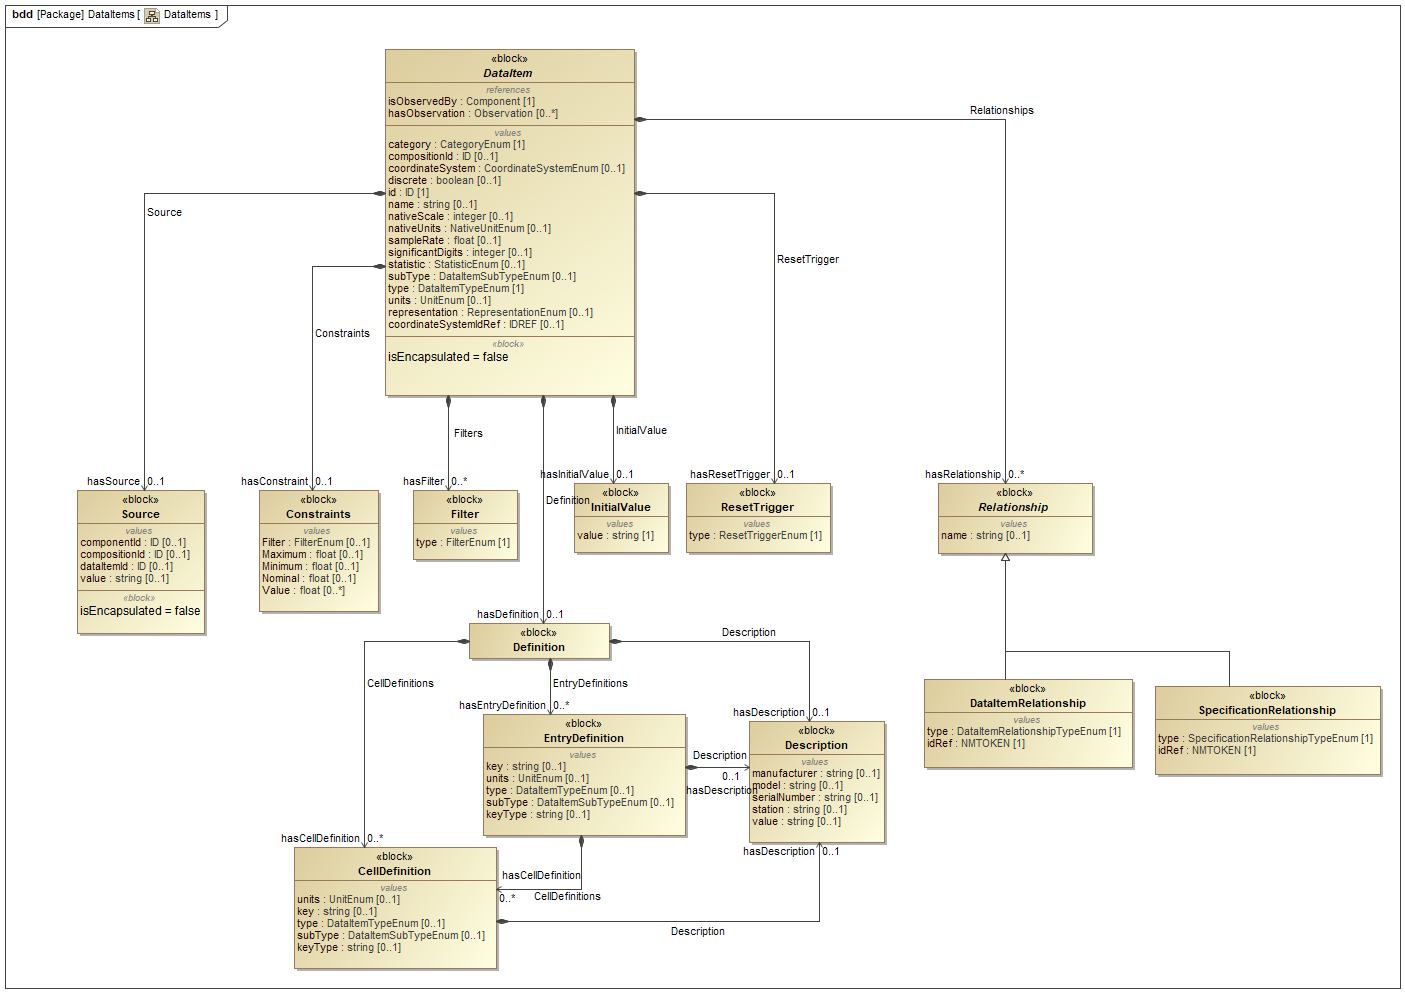
\includegraphics[width=1.0\textwidth]{figures/DataItems.png}
  \caption{DataItems Diagram}
  \label{fig:DataItems Diagram}
\end{figure}

\FloatBarrier


Note: See \fig{DataItems Schema Diagram} for XML schema.


\subsubsection{DataItem}
\label{sec:DataItem}



\block{DataItem} describes a piece of information reported about a piece of equipment.


\paragraph{Attributes of DataItem}\mbox{}
\label{sec:Attributes of DataItem}

\tbl{Attributes of DataItem} lists the attributes of \texttt{DataItem}.

\begin{table}[ht]
\centering 
  \caption{Attributes of DataItem}
  \label{table:Attributes of DataItem}
\tabulinesep=3pt
\begin{tabu} to 6in {|l|l|l|} \everyrow{\hline}
\hline
\rowfont\bfseries {Attribute} & {Type} & {Multiplicity} \\
\tabucline[1.5pt]{}

\property{category}[DataItem] & \texttt{CategoryEnum} & 1 \\
\property{compositionId}[DataItem] & \texttt{ID} & 0..1 \\
\property{coordinateSystem}[DataItem] & \texttt{CoordinateSystemEnum} & 0..1 \\
\property{discrete}[DataItem] & \texttt{boolean} & 0..1 \\
\property{id}[DataItem] & \texttt{ID} & 1 \\
\property{name}[DataItem] & \texttt{string} & 0..1 \\
\property{nativeScale}[DataItem] & \texttt{integer} & 0..1 \\
\property{nativeUnits}[DataItem] & \texttt{NativeUnitEnum} & 0..1 \\
\property{sampleRate}[DataItem] & \texttt{float} & 0..1 \\
\property{significantDigits}[DataItem] & \texttt{integer} & 0..1 \\
\property{statistic}[DataItem] & \texttt{StatisticEnum} & 0..1 \\
\property{subType}[DataItem] & \texttt{DataItemSubTypeEnum} & 0..1 \\
\property{type}[DataItem] & \texttt{DataItemTypeEnum} & 1 \\
\property{units}[DataItem] & \texttt{UnitEnum} & 0..1 \\
\property{representation}[DataItem] & \texttt{RepresentationEnum} & 0..1 \\
\property{coordinateSystemIdRef}[DataItem] & \texttt{IDREF} & 0..1 \\
\end{tabu}
\end{table}
\FloatBarrier

Descriptions for attributes of \block{DataItem}:

\begin{itemize}

\item \property{category}[DataItem] \newline Specifies the kind of information provided by a data item.

\texttt{CategoryEnum} Enumeration:

\begin{itemize}
\item \texttt{SAMPLE} \newline A \texttt{SAMPLE} is the reading of the value of a continuously variable or analog data value. A continuous value can be measured at any point-in-time and will always produce a result. 
\item \texttt{EVENT} \newline An \texttt{EVENT} is a data item representing a discrete piece of information from the piece of equipment. 
\item \texttt{CONDITION} \newline A \texttt{CONDITION} is a data item that communicates information about the health of a piece of equipment and its ability to function. 
\end{itemize}


\item \property{compositionId}[DataItem] \newline The identifier attribute of the \block{Composition} element that the reported data is most closely associated.

\item \property{coordinateSystem}[DataItem] \newline For measured values relative to a coordinate system like \block{POSITION}, the coordinate system being used may be reported.

\texttt{CoordinateSystemEnum} Enumeration:

\begin{itemize}
\item \texttt{MACHINE} \newline An unchangeable coordinate system that has machine zero as its origin. 
\item \texttt{WORK} \newline The coordinate system that represents the working area for a particular workpiece whose origin is shifted within the \texttt{MACHINE} coordinate system. If the \texttt{WORK} coordinates are not currently defined in the piece of equipment, the \texttt{MACHINE}
coordinates will be used. 
\end{itemize}


\item \property{discrete}[DataItem] \newline An indication signifying whether each value reported for the \gls{data entity} is significant and whether duplicate values are to be suppressed.

If a value is not defined for \property{discrete}, the default value \textbf{MUST} be \texttt{false}.

\item \property{id}[DataItem] \newline The unique identifier for this element.

\item \property{name}[DataItem] \newline The name of an element or a piece of equipment.

\item \property{nativeScale}[DataItem] \newline \block{nativeScale} \textbf{MAY} be used to convert the reported value to represent the original measured value.

\item \property{nativeUnits}[DataItem] \newline The native units of measurement for the reported value of the data item.

\texttt{NativeUnitEnum} Enumeration:

\begin{itemize}
\item \texttt{CENTIPOISE} \newline A measure of viscosity. 
\item \texttt{DEGREE/MINUTE} \newline Rotational velocity in degrees per minute. 
\item \texttt{FAHRENHEIT} \newline Temperature in Fahrenheit. 
\item \texttt{FOOT} \newline Feet. 
\item \texttt{FOOT/MINUTE} \newline Feet per minute. 
\item \texttt{FOOT/SECOND} \newline Feet per second. 
\item \texttt{FOOT/SECOND\^{}2} \newline Acceleration in feet per second squared. 
\item \texttt{FOOT\textunderscore 3D} \newline A point in space identified by X, Y, and Z positions and represented by a space-delimited set of numbers each expressed in feet. 
\item \texttt{GALLON/MINUTE} \newline Gallons per minute. 
\item \texttt{HOUR} \newline A measurement of time in hours. 
\item \texttt{INCH} \newline Inches. 
\item \texttt{INCH/MINUTE} \newline Inches per minute. 
\item \texttt{INCH/SECOND} \newline Inches per second. 
\item \texttt{INCH/SECOND\^{}2} \newline Acceleration in inches per second squared. 
\item \texttt{INCH\textunderscore POUND} \newline A measure of torque in inch pounds. 
\item \texttt{INCH\textunderscore 3D} \newline A point in space identified by X, Y, and Z positions and represented by a space-delimited set of numbers each expressed in inches. 
\item \texttt{KELVIN} \newline A measurement of temperature. 
\item \texttt{KILOWATT} \newline A measurement in kilowatt. 
\item \texttt{KILOWATT\textunderscore HOUR} \newline Kilowatt hours which is 3.6 mega joules. 
\item \texttt{LITER} \newline Measurement of volume of a fluid. 
\item \texttt{LITER/MINUTE} \newline Measurement of rate of flow of a fluid. 
\item \texttt{MILLIMETER/MINUTE} \newline Velocity in millimeters per minute. 
\item \texttt{MINUTE} \newline A measurement of time in minutes. 
\item \texttt{OTHER} \newline Unsupported units. 
\item \texttt{POUND} \newline US pounds. 
\item \texttt{POUND/INCH\^{}2} \newline Pressure in pounds per square inch (PSI). 
\item \texttt{RADIAN} \newline Angle in radians. 
\item \texttt{RADIAN/MINUTE} \newline Velocity in radians per minute. 
\item \texttt{RADIAN/SECOND} \newline Rotational acceleration in radian per second squared. 
\item \texttt{RADIAN/SECOND\^{}2} \newline Rotational acceleration in radian per second squared. 
\item \texttt{REVOLUTION/SECOND} \newline Rotational velocity in revolution per second. 
\item \texttt{BAR} \newline Pressure in Bar. 
\item \texttt{TORR} \newline Pressure in Torr. 
\item \texttt{MILLIMETER\textunderscore MERCURY} \newline Pressure in Millimeter of Mercury (mmHg). 
\item \texttt{PASCAL/MINUTE} \newline Pascal per minute. 
\end{itemize}


\item \property{sampleRate}[DataItem] \newline The rate at which successive samples of a data item are recorded by a piece of equipment.

\item \property{significantDigits}[DataItem] \newline The number of significant digits in the reported value.

\item \property{statistic}[DataItem] \newline Describes the type of statistical calculation performed on a series of data samples to provide the reported data value.

\texttt{StatisticEnum} Enumeration:

\begin{itemize}
\item \texttt{AVERAGE} \newline Mathematical Average value calculated for the data item during the calculation period. 
\item \texttt{KURTOSIS} \newline \textbf{DEPRECATED} in \textit{Version 1.6}. \sout{A measure of the "peakedness" of a probability distribution; i.e., the shape of the distribution curve.} 
\item \texttt{MAXIMUM} \newline Maximum or peak value recorded for the data item during the calculation period. 
\item \texttt{MEDIAN} \newline The middle number of a series of numbers. 
\item \texttt{MINIMUM} \newline Minimum value recorded for the data item during the calculation period. 
\item \texttt{MODE} \newline The number in a series of numbers that occurs most often. 
\item \texttt{RANGE} \newline Difference between the maximum and minimum value of a data item during the calculation period. Also represents Peak-to-Peak measurement in a waveform. 
\item \texttt{ROOT\textunderscore MEAN\textunderscore SQUARE} \newline Mathematical Root Mean Square (RMS) value calculated for the data item during the calculation period. 
\item \texttt{STANDARD\textunderscore DEVIATION} \newline Statistical Standard Deviation value calculated for the data item during the calculation period. 
\end{itemize}


\item \property{subType}[DataItem] \newline A sub-categorization of the data item \block{type}.

\item \property{type}[DataItem] \newline The type of either a \gls{structural element} or a \block{DataItem} being measured.

\item \property{units}[DataItem] \newline The unit of measurement for the reported value of the data item.

\texttt{UnitEnum} Enumeration:

\begin{itemize}
\item \texttt{AMPERE} \newline Amps 
\item \texttt{CELSIUS} \newline Degrees Celsius 
\item \texttt{COUNT} \newline A count of something. 
\item \texttt{DECIBEL} \newline Sound Level 
\item \texttt{DEGREE} \newline Angle in degrees 
\item \texttt{DEGREE\textunderscore 3D} \newline A space-delimited, floating-point representation of the angular rotation in degrees around the X, Y, and Z axes relative to a cartesian coordinate system respectively in order as A, B, and C. If any of the rotations is not known, it \textbf{MUST} be zero (0). 
\item \texttt{DEGREE/SECOND} \newline Angular degrees per second 
\item \texttt{DEGREE/SECOND\^{}2} \newline Angular acceleration in degrees per second squared 
\item \texttt{HERTZ} \newline Frequency measured in cycles per second 
\item \texttt{JOULE} \newline A measurement of energy. 
\item \texttt{KILOGRAM} \newline Kilograms 
\item \texttt{LITER} \newline Measurement of volume of a fluid 
\item \texttt{LITER/SECOND} \newline Liters per second 
\item \texttt{MICRO\textunderscore RADIAN} \newline Measurement of Tilt 
\item \texttt{MILLIMETER} \newline Millimeters 
\item \texttt{MILLIMETER\textunderscore 3D} \newline A point in space identified by X, Y, and Z positions and represented by a space-delimited set of numbers each expressed in millimeters. 
\item \texttt{MILLIMETER/REVOLUTION} \newline Millimeters per revolution. 
\item \texttt{MILLIMETER/SECOND} \newline Millimeters per second 
\item \texttt{MILLIMETER/SECOND\^{}2} \newline Acceleration in millimeters per second squared 
\item \texttt{NEWTON} \newline Force in Newtons 
\item \texttt{NEWTON\textunderscore METER} \newline Torque, a unit for force times distance. 
\item \texttt{OHM} \newline Measure of Electrical Resistance 
\item \texttt{PASCAL} \newline Pressure in Newtons per square meter 
\item \texttt{PASCAL\textunderscore SECOND} \newline Measurement of Viscosity 
\item \texttt{PERCENT} \newline Percentage 
\item \texttt{PH} \newline A measure of the acidity or alkalinity of a solution. 
\item \texttt{REVOLUTION/MINUTE} \newline Revolutions per minute 
\item \texttt{SECOND} \newline A measurement of time. 
\item \texttt{SIEMENS/METER} \newline A measurement of Electrical Conductivity 
\item \texttt{VOLT} \newline Volts 
\item \texttt{VOLT\textunderscore AMPERE} \newline The measurement of the apparent power in an electrical circuit, equal to the product of root-mean-square (RMS) voltage and RMS current (commonly referred to as VA). 
\item \texttt{VOLT\textunderscore AMPERE\textunderscore REACTIVE} \newline The measurement of reactive power in an AC electrical circuit (commonly referred to as VAR). 
\item \texttt{WATT} \newline Watts 
\item \texttt{WATT\textunderscore SECOND} \newline Measurement of electrical energy, equal to one Joule 
\item \texttt{REVOLUTION/SECOND} \newline Revolutions per second. 
\item \texttt{REVOLUTION/SECOND\^{}2} \newline Revolutions per second squared. 
\item \texttt{GRAM/CUBIC\textunderscore METER} \newline Gram per cubic meter. 
\item \texttt{CUBIC\textunderscore MILLIMETER} \newline Geometric volume in millimeters. 
\item \texttt{CUBIC\textunderscore MILLIMETER/SECOND} \newline Change of geometric volume per second. 
\item \texttt{CUBIC\textunderscore MILLIMETER/SECOND\^{}2} \newline Change in geometric volume per second squared. 
\item \texttt{MILLIGRAM} \newline Milligram. 
\item \texttt{MILLIGRAM/CUBIC\textunderscore MILLIMETER} \newline Milligram per cubic millimeter. 
\item \texttt{MILLILITER} \newline Milliliter. 
\item \texttt{COUNT/SECOND} \newline Counts per second. 
\item \texttt{PASCAL/SECOND} \newline Pascal per second. 
\item \texttt{UNIT\textunderscore VECTOR\textunderscore 3D} \newline A 3D Unit Vector.

Space delimited list of three floating point numbers. 
\end{itemize}


\item \property{representation}[DataItem] \newline Description of a means to interpret data consisting of multiple data points or samples reported as a single value.  

If \property{representation} is not specified, it \textbf{MUST} be determined to be \texttt{VALUE}.


\texttt{RepresentationEnum} Enumeration:

\begin{itemize}
\item \texttt{TIME\textunderscore SERIES} \newline A series of sampled data.

The data is reported for a specified number of samples and each sample is reported with a fixed period. 
\item \texttt{VALUE} \newline The measured value of the sample data.

If no \property{representation}[DataItem] is specified for a data item, the \property{representation}[DataItem] \textbf{MUST} be determined to be \texttt{VALUE}. 
\item \texttt{DATA\textunderscore SET} \newline The reported value(s) are represented as a set of \glspl{key-value pair}.

Each reported value in the \gls{data set} \textbf{MUST} have a unique key. 
\item \texttt{DISCRETE} \newline \textbf{DEPRECATED} as a \property{representation} in \textit{MTConnect Version. 1.5}. Replaced by the \property{discrete}[DataItem] attribute of a \block{DataItem}. 
\item \texttt{TABLE} \newline A \gls{table} is a two dimensional set of \glspl{key-value pair} where the \block{Entry} represents a row, and the value is a set of \gls{key-value pair} \block{Cell} elements. The \gls{table} follows the same behavior as the \gls{data set} for change tracking, clearing, and history. When an \block{Entry} changes, all \block{Cell} elements update as a single unit following the behavior of a \gls{data set}.

Note 1 to Entry: It is best to use the \block{Variable} \block{DataItem} \property{type} if the \block{Cell} elements represent multiple
semantic types.

Each \block{Entry} in the \gls{table} \textbf{MUST} have a unique key. Each \block{Cell} of each \block{Entry} in the \gls{table} \textbf{MUST} have a unique key.

See \textit{Section 5.6.5} of \citetitle{MTCPart3}, for a description of
\block{Entry} and \block{Cell} elements. 
\end{itemize}


\item \property{coordinateSystemIdRef}[DataItem] \newline The associated \block{CoordinateSystem} context for the \block{DataItem}.
\end{itemize}


\paragraph{Elements of DataItem}\mbox{}
\label{sec:Elements of DataItem}

\tbl{Elements of DataItem} lists the elements of \texttt{DataItem}.

\begin{table}[ht]
\centering 
  \caption{Elements of DataItem}
  \label{table:Elements of DataItem}
\tabulinesep=3pt
\begin{tabu} to 6in {|l|l|} \everyrow{\hline}
\hline
\rowfont\bfseries {Element} & {Multiplicity} \\
\tabucline[1.5pt]{}
\texttt{Source} & 0..1 \\
\texttt{Constraints} & 0..1 \\
\texttt{Filter} (organized by \block{Filters}) & 0..* \\
\texttt{InitialValue} & 0..1 \\
\texttt{ResetTrigger} & 0..1 \\
\texttt{Definition} & 0..1 \\
\texttt{Relationship} (organized by \block{Relationships}) & 0..* \\
\end{tabu}
\end{table}
\FloatBarrier


Descriptions for elements of \block{DataItem}:

\begin{itemize}

\item \block{Source} \newline \block{Source} identifies the \block{Component}, \block{DataItem}, or \block{Composition} representing the area of the piece of equipment from which a measured value originates.

\item \block{Constraints} \newline \block{Constraints} \glspl{organize} a set of expected values that can be reported for this \block{DataItem}.

\item \block{Filters} \newline \block{Filters} \glspl{organize} the \block{Filter} elements associated with this \block{DataItem} element. 

\item \block{InitialValue} \newline \block{InitialValue} defines the starting value for a data item as well as the value to be set for the data item after a reset event.

\item \block{ResetTrigger} \newline \block{ResetTrigger} identifies the type of event that may cause a reset to occur.

\item \block{Definition} \newline The \block{Definition} defines the meaning of \block{Entry} and \block{Cell} elements associated with the \block{DataItem} when the \property{representation} is either \block{DATA} or \block{TABLE}.

\item \block{Relationships} \newline \block{Relationships} \glspl{organize} one or more \block{DataItemRelationship} and \block{SpecificationRelationship}.
\end{itemize}


